\documentclass[12pt]{exam}		%Doc : https://mirrors.ircam.fr/pub/CTAN/macros/latex/contrib/exam/examdoc.pdf
\printanswers					%Comment this line to hide the answers 
\usepackage[utf8]{inputenc}
\usepackage[T1]{fontenc}
\usepackage[french]{babel}      %Originally for french document, change to english or relevant language

\usepackage{amsmath,amssymb}
\usepackage{multicol}
\usepackage[dvipsnames]{xcolor}
\usepackage[shortlabels]{enumitem}
\usepackage{tikz}
	\usetikzlibrary{fadings}
	\usetikzlibrary{calc}
	
\usepackage{tkz-tab}
\usepackage{pgfplots}

%Format Header and footer
\pagestyle{headandfoot}
\header{\footnotesize Class\\Id number}{\Large\textbf{Name}}
\headrule
\footrule
\setlength{\columnsep}{0.25cm}
%\setlength{\columnseprule}{1pt}
\footer{}{Page \thepage}{}
%\extrafootheight{-2cm}

% Change section command behaviour
\usepackage{titlesec}
\titleformat{\section}[frame]{\Huge\bfseries\filright}{}{2mm}{\centering Chemistry 107 :\ }

% Add a watermark if answers are shown
%\ifprintanswers
%\usepackage{draftwatermark}
%\SetWatermarkColor{red!30}
%\SetWatermarkScale{5}
%\SetWatermarkText{Solution}     %Watermark text
%\fi

%Format the name of each exercise
\qformat{\textbf{Exercice \thequestion~:}\hfill}
\extrawidth{1.5cm}

\begin{document}
\section{Exam 3A}

\noindent The 100 pts exam consists of 10 questions and students have 2 hours to complete the exam.
Answers must be written in the box provided or else no credit is provided. Use the empty
space provided to do your work. A periodic table and formulas are provided at the end. Additional
scratch paper will be provided. Fill in your name along with your student ID number.
\\

\noindent\textbf{Problem 1: True/False } Determine whether the statement is true or false. (10 pts)
\\
\begin{enumerate}[(a)]
\item The theoretical yield is determined based on the amount of the
  limiting reagent. %True
\item[]\tikz[baseline=1ex]\draw (0,0) rectangle (17cm,5ex);
\item The mass before and after the reaction is conserverd. %True
\item[]\tikz[baseline=1ex]\draw (0,0) rectangle (17cm,5ex);
\item An example of an exothermic reaction is melting ice into
  water. %False
\item[]\tikz[baseline=1ex]\draw (0,0) rectangle (17cm,5ex);
\item Suppose two objects are at thermal equilibrium. Then, there is no flow of
  heat between the objects. %False
\item[]\tikz[baseline=1ex]\draw (0,0) rectangle (17cm,5ex);
\item Fluorine has the highest electronegativity. %True
\item[]\tikz[baseline=1ex]\draw (0,0) rectangle (17cm,5ex);
\item Exothermic reactions releases heat. %True
\item[]\tikz[baseline=1ex]\draw (0,0) rectangle (17cm,5ex);
\item The Bohr model of an atom can accurately describe the atomic spectra
  of large atoms. %False
\item[]\tikz[baseline=1ex]\draw (0,0) rectangle (17cm,5ex);
\item When an electron in the hydrogen atom falls from $n=2$ to $n=1$,
  then light is being absorbed. %False
\item[]\tikz[baseline=1ex]\draw (0,0) rectangle (17cm,5ex);
\item In a continuous spectrum, the energy of the electron is not quantized.
  %True
\item[]\tikz[baseline=1ex]\draw (0,0) rectangle (17cm,5ex);
\end{enumerate}

\newpage

\noindent\textbf{Problem 2: Thermal Equilibrium} (12 pts)
\vspace{0.2in}

\noindent (a) Suppose 150.0g of water at $95^\circ$C is mixed with
50.00g of water at $15^\circ$C. The specific heat of water is 4.184 J/(g $^\circ$C).
At thermal equilibrium, what is the final temperature? Report to 4
significant figures.

\vspace{2.5in}

\tikz[baseline=1ex]\draw (0,0) rectangle (17cm,5ex);
\\

\noindent (b) Describe using illustrations and/or equations to show how thermal equilibrium
is achieved.
\\

\tikz[baseline=1ex]\draw (0,0) rectangle (17.5cm,55ex);

\vspace{0.3in}

\newpage

\noindent\textbf{Problem 3: Nomenclature} Provide either the molecular formula or
compound name for the following. (6 pts)
\\
\begin{enumerate}[(a)]
\item Sulfur monoxide %SO
\item[]\tikz[baseline=1ex]\draw (0,0) rectangle (17cm,5ex);
\item MgCrO$_4$ %Magnesium chromate
\item[]\tikz[baseline=1ex]\draw (0,0) rectangle (17cm,5ex);
\item HClO$_2$ %Chlorous acid
\item[]\tikz[baseline=1ex]\draw (0,0) rectangle (17cm,5ex);
\item Cu$_3$(PO$_4$)$_2$ %Copper(II) phosphate
\item[]\tikz[baseline=1ex]\draw (0,0) rectangle (17cm,5ex);
\item H$_2$CO$_3$ %Carbonic acid
\item[]\tikz[baseline=1ex]\draw (0,0) rectangle (17cm,5ex);
\item Chlorine trifluoride %ClF3
\item[]\tikz[baseline=1ex]\draw (0,0) rectangle (17cm,5ex);
\end{enumerate}

\newpage

\noindent\textbf{Problem 4: Preparing Solutions} A scientist is making
CuSO$_4$ solution for his experiments. The available solute is CuSO$_4\cdot$5H$_2$O
(Molar mass = 249.68 g/mol). Answer the following questions and report to 3
significant figures. (8 pts)
\\
\begin{enumerate}[(a)]
\item The scientist prepares 2L stock solution of 3M CuSO$_4$. Determine what
  mass (in g) of CuSO$_4\cdot$5H$_2$O needed to prepare the solution.
  \vspace{1.75in}
\item[]\tikz[baseline=1ex]\draw (0,0) rectangle (17cm,5ex);
\item The scientist only has 250mL volumetric flask available to dilute
  the 3M CuSO$_4$ stock solution to 0.75M CuSO$_5$ What volume in L of stock solution
  is needed to dilute to prepare 250.mL of 1.5M CaCl$_2$?
  \vspace{1.75in}
\item[]\tikz[baseline=1ex]\draw (0,0) rectangle (17cm,5ex);
\end{enumerate}

\newpage

\noindent\textbf{Problem 5: Photosynthesis - the Chloroplast} Photosynthesis
is a vital process providing organisms oxygen and food. Plants performs this vital
process using a protein called chlorophyll a. The protein absorbs mainly light at
430nm (violet) and and 662nm (red). Answer the following questions and report to
3 significant figures. (8 pts)

\begin{enumerate}[(a)]
\item Determine the energy in J of the violet (430nm) and red light (662nm) that
  chlorophyll a absorbs.
  \vspace{2.5in}
\item[]\tikz[baseline=1ex]\draw (0,0) rectangle (17cm,5ex);
\item How much energy is contained in one mole of photons for violet and red lights?
  \vspace{2.5in}
\item[]\tikz[baseline=1ex]\draw (0,0) rectangle (17cm,5ex);
\end{enumerate}

\newpage

\noindent\textbf{Problem 6: Energy from a Laser} In 2021, HiLASE Center broke the world
record developing the strongest high-energy laser that emits a wavelength of 1030nm.
Answer the following questions and report to 3 significant figures. (12 pts)

\begin{enumerate}[(a)]
\item Determine the energy of a single photon from 1030nm.
  \vspace{1.75in}
\item[]\tikz[baseline=1ex]\draw (0,0) rectangle (17cm,5ex);
\item A single laser pulse emits 145 Joules of energy. Determine how many
  photons that is.
  \vspace{1.75in}
\item[]\tikz[baseline=1ex]\draw (0,0) rectangle (17cm,5ex);
\item Compute the energy in J/mol of a mole of photon at 1030nm. Compare this energy
  to part b).
  \vspace{1.75in}
\item[]\tikz[baseline=1ex]\draw (0,0) rectangle (17cm,5ex);
\end{enumerate}

\newpage

\noindent\textbf{Problem 7: Drawing Lewis Structures}
Draw the Lewis structures for the following compounds, identify the
geometric shape, and whether the compound is polar or nonpolar. If there
are resonance structures, then include them in your answer.(12 pts)

\begin{enumerate}[(a)]
\item CO$_2$
\item[]\tikz[baseline=1ex]\draw (0,0) rectangle (17.5cm,34ex);
\item SCN$^-$ 
\item[]\tikz[baseline=1ex]\draw (0,0) rectangle (17.5cm,34ex);
\item BF$_3$
\item[]\tikz[baseline=1ex]\draw (0,0) rectangle (17.5cm,34ex);
%\item NH$_3$
%\item[]\tikz[baseline=1ex]\draw (0,0) rectangle (17.5cm,35ex);
%\item PO$_4^{3-}$
%\item[]\tikz[baseline=1ex]\draw (0,0) rectangle (17.5cm,35ex);
%\item SO$_4^{2-}$
%\item[]\tikz[baseline=1ex]\draw (0,0) rectangle (17.5cm,35ex);
\end{enumerate}

\newpage

\noindent\textbf{Problem 8: Periodic Properties} Rank the following
periodic properties. (8 pts)

\begin{enumerate}[(a)]
\item Rank elements from highest to lowest first ionization energy:
  F, Li, He, Mg, I %He, F, I, Li, Mg
\item[]\tikz[baseline=1ex]\draw (0,0) rectangle (17cm,5ex);
\item Rank elements from highest to lowest electronegativity:
  Li, Be, Se, O, F %F, O, Se, Be, Li
\item[]\tikz[baseline=1ex]\draw (0,0) rectangle (17cm,5ex);
\item Rank elements from largest to smallest atomic radius:
  He, H, K, F, I %K, I, F, H, He
\item[]\tikz[baseline=1ex]\draw (0,0) rectangle (17cm,5ex);
\item Ranking ions from largest to smeallest atomic radius:
  N$^{3-}$, I$^-$, Li$^+$, F$^-$, O$^{2-}$ % I-, N3-, O2-, F-, Li+
\item[]\tikz[baseline=1ex]\draw (0,0) rectangle (17cm,5ex);
\end{enumerate}

\vspace{0.5in}

\noindent\textbf{Problem 9: Electron Configuration} Determine the electron
configurations for the following. (14 pts)

\begin{enumerate}[(a)]
\item Mg % [Ne]2s2
\item[]\tikz[baseline=1ex]\draw (0,0) rectangle (17cm,5ex);
\item S % [Ne]3s2 3p4
\item[]\tikz[baseline=1ex]\draw (0,0) rectangle (17cm,5ex);
\item Al$^{3+}$ %[Ne]
\item[]\tikz[baseline=1ex]\draw (0,0) rectangle (17cm,5ex);
\item Cr % [Ar]4s1 3d5
\item[]\tikz[baseline=1ex]\draw (0,0) rectangle (17cm,5ex);
\item Zn$^{2+}$ % [Ar]3d10
\item[]\tikz[baseline=1ex]\draw (0,0) rectangle (17cm,5ex);
\item Fe$^{2+}$ % [Ar]3d10
\item[]\tikz[baseline=1ex]\draw (0,0) rectangle (17cm,5ex);
\item Ag$^+$ % [Ar]3d10
\item[]\tikz[baseline=1ex]\draw (0,0) rectangle (17cm,5ex);
\end{enumerate}
\newpage

\noindent\textbf{Problem 10: Combustion Reaction} Propane (C$_3$H$_8$) is a colorless and odorless gas.
It is commonly used for grilling. Per year, the US uses approximately 10.0 billion
($\times 10^{9}$) gallons of propane per year. This is equivalent to $1.86\times 10^{10}$ kg
propane. Answer the following questions and report to 3 significant figures. (10 pts)
\\
\begin{enumerate}[(a)]
\item Write the balanced chemical equation including states of the combustion reaction of propane
  (C$_3$H$_8$).
\item[]\tikz[baseline=1ex]\draw (0,0) rectangle (17cm,5ex);
\item In the presence of excess oxygen gas, determine
  the amount of carbon dioxide is produced in g? Report in scientific notation.
  \vspace{2in}
\item[]\tikz[baseline=1ex]\draw (0,0) rectangle (17cm,5ex);
\item The combustion reaction of methane releases 2220.0 kJ/mol. Is this an exothermic or
  endothermic reaction? How much heat is generated per year from propane usage? Report in
  scientific notation.
  \vspace{2in}
\item[]\tikz[baseline=1ex]\draw (0,0) rectangle (17cm,5ex);
\end{enumerate}

%\newpage
%
%\noindent\textbf{Problem 11: Meaning of Chemical Equation} Souring of wine
%occurs when ethanol (C$_2$H$_5$OH) is converted to acetic acid (CH$_3$COOH)
%by oxygen (O$_2$):
%\\
%
%\noindent
%C$_2$H$_5$OH(l) + O$_2$(g) $\rightarrow$ CH$_3$COOH(aq) + H$_2$O(l).
%\\
%
%\noindent
%Answer the following questions and report to 2 significant
%figures. (12 pts)
%\\
%
%\begin{enumerate}[(a)]
%\item Suppose there is 70.g ethanol in a 1.0L bottle of wine and the
%  bottle has a defective seal. What mass of oxygen must leak into the bottle to
%  completely react with ethanol?
%  \vspace{1.75in}
%\item[]\tikz[baseline=1ex]\draw (0,0) rectangle (17cm,5ex);
%\item If 27g acetic acid was found in the wine bottle, how much of ethanol
%  in g was converted?
%  \vspace{1.75in}
%\item[]\tikz[baseline=1ex]\draw (0,0) rectangle (17cm,5ex);
%\item Based on part b), how much ethanol in g is leftover in the wine bottle?
%  \vspace{1.75in}
%\item[]\tikz[baseline=1ex]\draw (0,0) rectangle (17cm,5ex);
%\end{enumerate}

\newpage

\appendix

\section{Appendix 1 - Periodic Table}

\begin{center}
  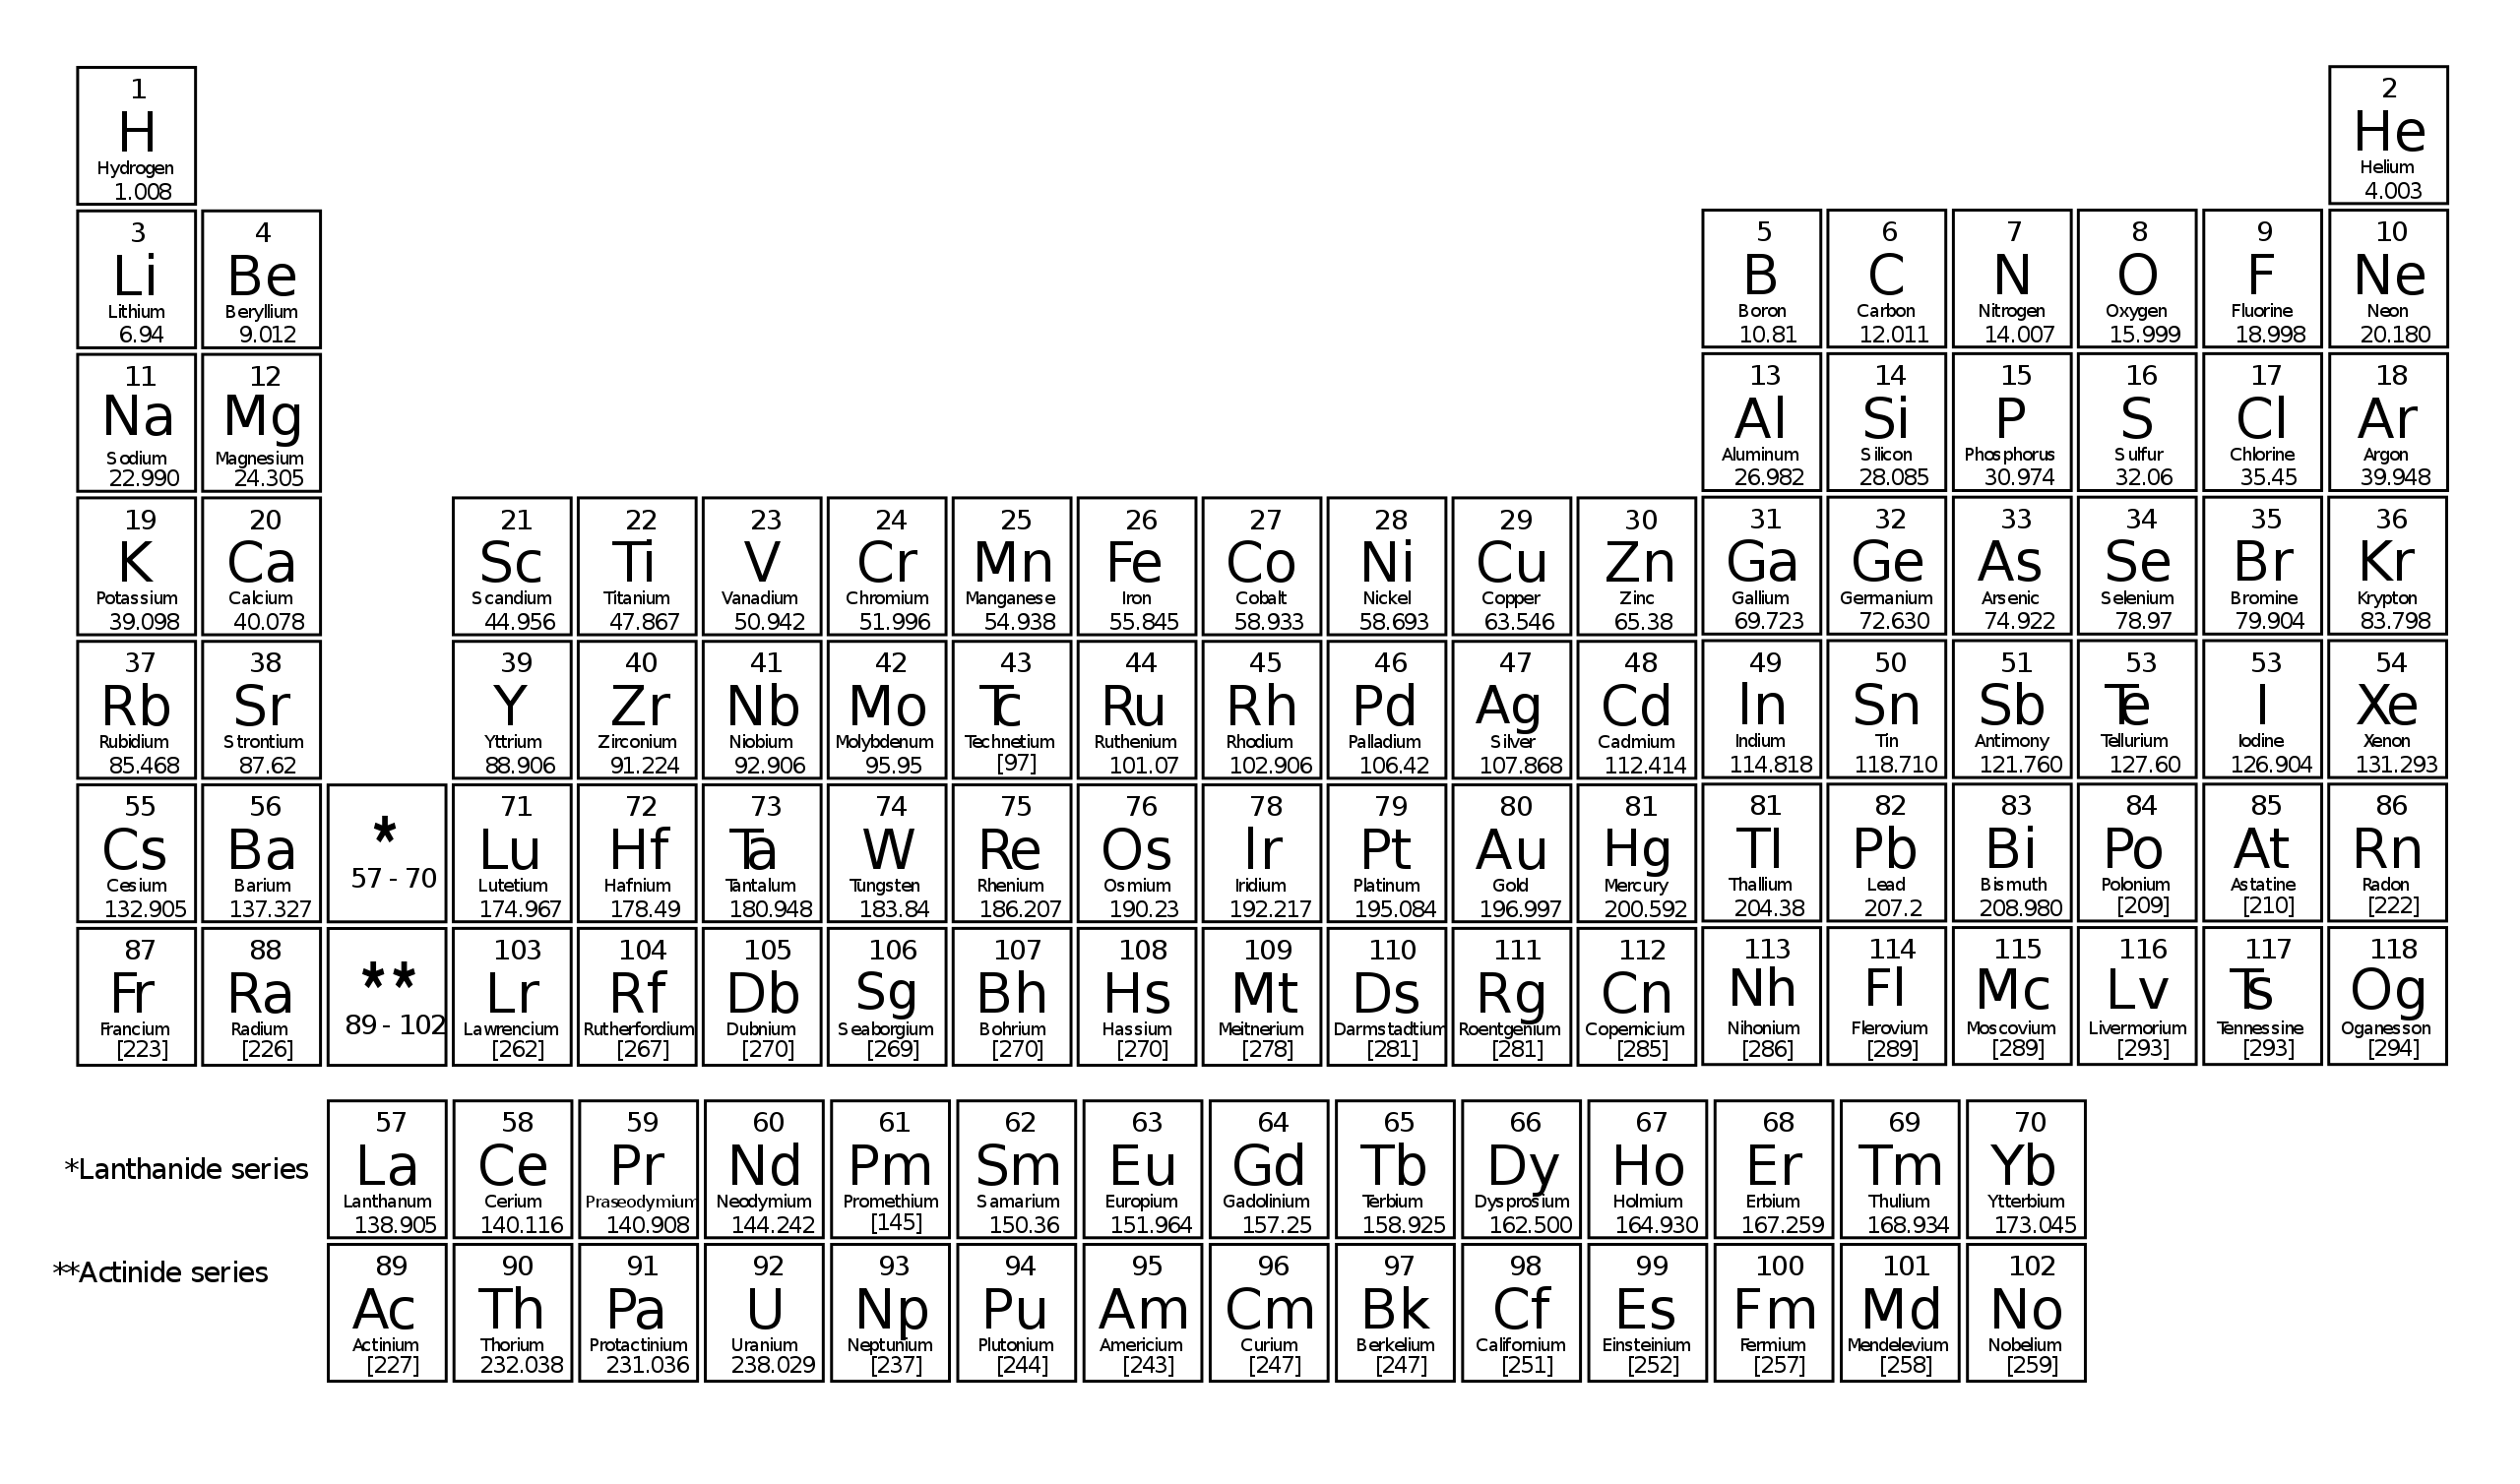
\includegraphics[scale=0.24,angle=90]{periodic_table}
\end{center}

\section{Apppendix 2 - Formulas and Constants}

\begin{align*}
  q = & mC\Delta T \\
  E = & \frac{hc}{\lambda} = h\nu \\
  h = & 6.626 \times 10^{-34} \text{J s} \\
  c = & \lambda \nu \\
  c = & 3.00 \times 10^8 \text{m/s} \\
  N_A = & 6.022\times 10^{23}
\end{align*}
\end{document}
